\documentclass[10pt,ignorenonframetext,compress, aspectratio=169]{beamer}
\setbeamertemplate{caption}[numbered]
\setbeamertemplate{caption label separator}{: }
\setbeamercolor{caption name}{fg=normal text.fg}
\beamertemplatenavigationsymbolsempty
\usepackage{lmodern}
\usepackage{amssymb,amsmath,mathtools}
\usepackage{ifxetex,ifluatex}
\usepackage{fixltx2e} % provides \textsubscript
\ifnum 0\ifxetex 1\fi\ifluatex 1\fi=0 % if pdftex
  \usepackage[T1]{fontenc}
  \usepackage[utf8]{inputenc}
\else % if luatex or xelatex
  \ifxetex
    \usepackage{mathspec}
  \else
    \usepackage{fontspec}
  \fi
  %%\defaultfontfeatures{Ligatures=TeX,Scale=MatchLowercase}
  \defaultfontfeatures{Scale=MatchLowercase}
\fi
\usetheme[]{metropolis}
% use upquote if available, for straight quotes in verbatim environments
\IfFileExists{upquote.sty}{\usepackage{upquote}}{}
% use microtype if available
\IfFileExists{microtype.sty}{%
\usepackage{microtype}
\UseMicrotypeSet[protrusion]{basicmath} % disable protrusion for tt fonts
}{}
\newif\ifbibliography
\usepackage{color}
\usepackage{fancyvrb}
\newcommand{\VerbBar}{|}
\newcommand{\VERB}{\Verb[commandchars=\\\{\}]}
\DefineVerbatimEnvironment{Highlighting}{Verbatim}{commandchars=\\\{\}}
% Add ',fontsize=\small' for more characters per line
\usepackage{framed}
\definecolor{shadecolor}{RGB}{248,248,248}
\newenvironment{Shaded}{\begin{snugshade}}{\end{snugshade}}
\newcommand{\KeywordTok}[1]{\textcolor[rgb]{0.13,0.29,0.53}{\textbf{{#1}}}}
\newcommand{\DataTypeTok}[1]{\textcolor[rgb]{0.13,0.29,0.53}{{#1}}}
\newcommand{\DecValTok}[1]{\textcolor[rgb]{0.00,0.00,0.81}{{#1}}}
\newcommand{\BaseNTok}[1]{\textcolor[rgb]{0.00,0.00,0.81}{{#1}}}
\newcommand{\FloatTok}[1]{\textcolor[rgb]{0.00,0.00,0.81}{{#1}}}
\newcommand{\ConstantTok}[1]{\textcolor[rgb]{0.00,0.00,0.00}{{#1}}}
\newcommand{\CharTok}[1]{\textcolor[rgb]{0.31,0.60,0.02}{{#1}}}
\newcommand{\SpecialCharTok}[1]{\textcolor[rgb]{0.00,0.00,0.00}{{#1}}}
\newcommand{\StringTok}[1]{\textcolor[rgb]{0.31,0.60,0.02}{{#1}}}
\newcommand{\VerbatimStringTok}[1]{\textcolor[rgb]{0.31,0.60,0.02}{{#1}}}
\newcommand{\SpecialStringTok}[1]{\textcolor[rgb]{0.31,0.60,0.02}{{#1}}}
\newcommand{\ImportTok}[1]{{#1}}
\newcommand{\CommentTok}[1]{\textcolor[rgb]{0.56,0.35,0.01}{\textit{{#1}}}}
\newcommand{\DocumentationTok}[1]{\textcolor[rgb]{0.56,0.35,0.01}{\textbf{\textit{{#1}}}}}
\newcommand{\AnnotationTok}[1]{\textcolor[rgb]{0.56,0.35,0.01}{\textbf{\textit{{#1}}}}}
\newcommand{\CommentVarTok}[1]{\textcolor[rgb]{0.56,0.35,0.01}{\textbf{\textit{{#1}}}}}
\newcommand{\OtherTok}[1]{\textcolor[rgb]{0.56,0.35,0.01}{{#1}}}
\newcommand{\FunctionTok}[1]{\textcolor[rgb]{0.00,0.00,0.00}{{#1}}}
\newcommand{\VariableTok}[1]{\textcolor[rgb]{0.00,0.00,0.00}{{#1}}}
\newcommand{\ControlFlowTok}[1]{\textcolor[rgb]{0.13,0.29,0.53}{\textbf{{#1}}}}
\newcommand{\OperatorTok}[1]{\textcolor[rgb]{0.81,0.36,0.00}{\textbf{{#1}}}}
\newcommand{\BuiltInTok}[1]{{#1}}
\newcommand{\ExtensionTok}[1]{{#1}}
\newcommand{\PreprocessorTok}[1]{\textcolor[rgb]{0.56,0.35,0.01}{\textit{{#1}}}}
\newcommand{\AttributeTok}[1]{\textcolor[rgb]{0.77,0.63,0.00}{{#1}}}
\newcommand{\RegionMarkerTok}[1]{{#1}}
\newcommand{\InformationTok}[1]{\textcolor[rgb]{0.56,0.35,0.01}{\textbf{\textit{{#1}}}}}
\newcommand{\WarningTok}[1]{\textcolor[rgb]{0.56,0.35,0.01}{\textbf{\textit{{#1}}}}}
\newcommand{\AlertTok}[1]{\textcolor[rgb]{0.94,0.16,0.16}{{#1}}}
\newcommand{\ErrorTok}[1]{\textcolor[rgb]{0.64,0.00,0.00}{\textbf{{#1}}}}
\newcommand{\NormalTok}[1]{{#1}}
\usepackage{graphicx,grffile}
\makeatletter
\def\maxwidth{\ifdim\Gin@nat@width>\linewidth\linewidth\else\Gin@nat@width\fi}
\def\maxheight{\ifdim\Gin@nat@height>\textheight0.8\textheight\else\Gin@nat@height\fi}
\makeatother
% Scale images if necessary, so that they will not overflow the page
% margins by default, and it is still possible to overwrite the defaults
% using explicit options in \includegraphics[width, height, ...]{}
\setkeys{Gin}{width=\maxwidth,height=\maxheight,keepaspectratio}

% Prevent slide breaks in the middle of a paragraph:
\widowpenalties 1 10000
\raggedbottom

\AtBeginPart{
  \let\insertpartnumber\relax
  \let\partname\relax
  \frame{\partpage}
}
\AtBeginSection{
  \ifbibliography
  \else
    \let\insertsectionnumber\relax
    \let\sectionname\relax
    \frame{\sectionpage}
  \fi
}
\AtBeginSubsection{
  \let\insertsubsectionnumber\relax
  \let\subsectionname\relax
  \frame{\subsectionpage}
}

\setlength{\parindent}{0pt}
\setlength{\parskip}{6pt plus 2pt minus 1pt}
\setlength{\emergencystretch}{3em}  % prevent overfull lines
\providecommand{\tightlist}{%
  \setlength{\itemsep}{0pt}\setlength{\parskip}{0pt}}
\setcounter{secnumdepth}{0}

%% GLS Added
% Textcomp for various common symbols
\usepackage{textcomp}

\usepackage{booktabs}

% Creative Commons Icons
\usepackage[scale=1]{ccicons}

\newenvironment{centrefig}{\begin{figure}\centering}{\end{figure}}
\newcommand{\columnsbegin}{\begin{columns}}
\newcommand{\columnsend}{\end{columns}}
\newcommand{\centreFigBegin}{\begin{figure}\centering}
\newcommand{\centreFigEnd}{\end{figure}}
%%

\DefineVerbatimEnvironment{Highlighting}{Verbatim}{commandchars=\\\{\}, fontsize=\tiny}
% make console-output smaller:
\makeatletter
\def\verbatim{\tiny\@verbatim \frenchspacing\@vobeyspaces \@xverbatim}
\makeatother
\setlength{\parskip}{0pt}
\setlength{\OuterFrameSep}{-4pt} % was -4pt
\makeatletter
\preto{\@verbatim}{\topsep=-10pt \partopsep=-10pt} % were -10pt
\makeatother

\title{Basic Ordination}
\author{Gavin L. Simpson}
\date{U Adelaide 2017 • Feb 13--17 2017}

\begin{document}
\frame{\titlepage}

\section{Introduction}\label{introduction}

\begin{frame}{Introduction}

\begin{itemize}
\tightlist
\item
  \alert{Ordination} comes from the German word \emph{ordnung}, meaning
  to put things in order
\item
  This is exactly what we we do in ordination --- we arrange our samples
  along gradients by fitting lines and planes through the data that
  describe the main patterns in those data
\item
  Linear and unimodal methods
\item
  Principle Components Analysis (PCA) is a linear method --- most useful
  for environmental data or sometimes with species data and short
  gradients
\item
  Correspondence Analysis (CA) is a unimodal method --- most useful for
  species data, especially where non-linear responses are observed
\end{itemize}

\end{frame}

\section{Principal Components
Analysis}\label{principal-components-analysis}

\begin{frame}{Ordination}

\begin{itemize}
\tightlist
\item
  Regression gives us a basis from which to work
\item
  Instead of doing many regressions, do one with all the species data
  once
\item
  Only now we don't have any explanatory variables, we wish to uncover
  these underlying gradients
\item
  PCA fits a line through our cloud of data in such a way that it
  maximises the variance in the data captured by that line
  (i.e.\textasciitilde{}minimises the distance between the fitted line
  and the observations)
\item
  Then we fit a second line to form a plane, and so on, until we have
  one PCA line or axis for each of our species
\item
  Each of these subsequent axes is uncorrelated with previous axes ---
  they are \alert{orthogonal} --- so the variance each axis explains is
  uncorrelated
\end{itemize}

\end{frame}

\begin{frame}{Principal Components Analysis}

\begin{figure}[htbp]
\centering
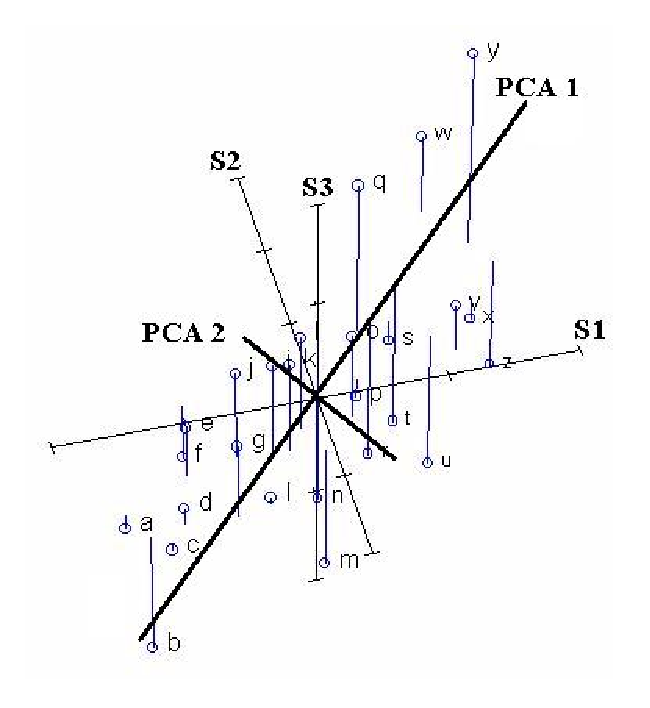
\includegraphics{pca_example_figure.pdf}
\caption{}
\end{figure}

\end{frame}

\begin{frame}{Vegetation in lichen pastures --- PCA}

Data are cover values of 44 understorey species recorded at 24 locations
in lichen pastures within dry \emph{Pinus sylvestris} forests

\begin{center}\includegraphics[width=0.7\linewidth]{01-basic-ordination_files/figure-beamer/vare-pca-1-1} \end{center}

\end{frame}

\begin{frame}{Vegetation in lichen pastures --- PCA biplots}

\columnsbegin
\column{0.5\linewidth}

\begin{itemize}
\tightlist
\item
  Have two sets of scores

  \begin{itemize}
  \tightlist
  \item
    Species scores
  \item
    Site scores \textbackslash{}end\{enumerate\}
  \end{itemize}
\item
  Sample (species) points plotted close together have similar species
  compositions (occur together)
\item
  In PCA, species scores often drawn as arrows --- point in direction of
  increasing abundance
\item
  Species arrows with small angles to an axis are highly correlated with
  that axis
\end{itemize}

\column{0.5\linewidth}

\begin{center}\includegraphics[width=0.7\linewidth]{01-basic-ordination_files/figure-beamer/vare-pca-2-1} \end{center}

\columnsend

\end{frame}

\begin{frame}[fragile]{Eigenvalues}

Eigenvalues \(\lambda\) are the amount of variance (inertia) explained
by each axis

\begin{Shaded}
\begin{Highlighting}[]
\KeywordTok{head}\NormalTok{(}\KeywordTok{eigenvals}\NormalTok{(pca), 6L)}
\end{Highlighting}
\end{Shaded}

\begin{verbatim}
     PC1      PC2      PC3      PC4      PC5      PC6 
8.602826 5.133623 4.575623 3.713926 3.244925 2.779195 
\end{verbatim}

\begin{Shaded}
\begin{Highlighting}[]
\KeywordTok{screeplot}\NormalTok{(pca, }\DataTypeTok{bstick =} \OtherTok{TRUE}\NormalTok{, }\DataTypeTok{type =} \StringTok{"l"}\NormalTok{, }\DataTypeTok{main =} \OtherTok{NULL}\NormalTok{)}
\end{Highlighting}
\end{Shaded}

\begin{center}\includegraphics[width=0.7\linewidth]{01-basic-ordination_files/figure-beamer/vare-pca-3-1} \end{center}

\end{frame}

\section{Correspondence Analysis}\label{correspondence-analysis}

\begin{frame}{Correspondence Analysis}

\end{frame}

\begin{frame}{Vegetation in lichen pastures --- CA biplots}

\columnsbegin
\column{0.5\linewidth}

\begin{itemize}
\tightlist
\item
  Have two sets of scores

  \begin{enumerate}
  \def\labelenumi{\arabic{enumi}.}
  \tightlist
  \item
    Species scores
  \item
    Site scores
  \end{enumerate}
\item
  Sample (species) points plotted close together have similar species
  compositions (occur together)
\item
  In CA, species scores drawn as points --- this is the fitted optima
  along the gradients
\item
  Abundance of species declines in concentric circles away from the
  optima
\end{itemize}

\column{0.5\linewidth}

\begin{center}\includegraphics[width=0.7\linewidth]{01-basic-ordination_files/figure-beamer/vare-ca-1-1} \end{center}

\columnsend

\end{frame}

\begin{frame}{Vegetation in lichen pastures --- CA biplots}

\begin{itemize}
\tightlist
\item
  Species scores plotted as weighted averages of site scores, or
\item
  Site scores plotted as weighted averages of species scores, or
\item
  A symmetric plot
\end{itemize}

\begin{center}\includegraphics[width=0.95\linewidth]{01-basic-ordination_files/figure-beamer/vare-ca-2-1} \end{center}

\end{frame}

\section{Vegan usage}\label{vegan-usage}

\begin{frame}[fragile]{Vegan basics}

\begin{itemize}
\tightlist
\item
  The majority of vegan functions work with a single vector, or more
  commonly an entire data frame
\item
  This data frame may contain the species abundances
\item
  Where subsidiary data is used/required, these two are supplied as data
  frames
\item
  For example; the environmental constraints in a CCA
\item
  It is not a problem if you have all your data in a single file/object;
  just subset it into two data frames after reading it into R
\end{itemize}

\begin{Shaded}
\begin{Highlighting}[]
\NormalTok{spp <-}\StringTok{ }\NormalTok{allMyData[, }\DecValTok{1}\NormalTok{:}\DecValTok{20}\NormalTok{] ## columns 1-20 contain the species data}
\NormalTok{env <-}\StringTok{ }\NormalTok{allMyData[, }\DecValTok{21}\NormalTok{:}\DecValTok{26}\NormalTok{] ## columns 21-26 contain the environmental data}
\end{Highlighting}
\end{Shaded}

\end{frame}

\begin{frame}[fragile]{Simple vegan usage}

First we start with a simple correspondence analysis (CA) to illustrate
the basic features

Here I am using one of the in-built data sets on lichen pastures

For various reasons to fit a CA we use the \texttt{cca()} function

Store the fitted CA in \texttt{ca1} and print it to view the results

\begin{Shaded}
\begin{Highlighting}[]
\NormalTok{ca1 <-}\StringTok{ }\KeywordTok{cca}\NormalTok{(varespec)}
\NormalTok{ca1}
\end{Highlighting}
\end{Shaded}

\begin{verbatim}
Call: cca(X = varespec)

              Inertia Rank
Total           2.083     
Unconstrained   2.083   23
Inertia is mean squared contingency coefficient 

Eigenvalues for unconstrained axes:
   CA1    CA2    CA3    CA4    CA5    CA6    CA7    CA8 
0.5249 0.3568 0.2344 0.1955 0.1776 0.1216 0.1155 0.0889 
(Showed only 8 of all 23 unconstrained eigenvalues)
\end{verbatim}

\end{frame}

\begin{frame}[fragile]{\texttt{scores()} \& \texttt{scaling} in
\texttt{cca()}, \texttt{rda()}}

\begin{itemize}
\tightlist
\item
  When we draw the results of many ordinations we display 2 or more sets
  of data
\item
  Can't display all of these and maintain relationships between the
  scores
\item
  Solution; scale one set of scores relative to the other
\item
  Controlled via the \texttt{scaling} argument

  \begin{itemize}
  \tightlist
  \item
    \texttt{scaling\ =\ 1} --- Focus on species, scale site scores by
    \(\lambda_i\)
  \item
    \texttt{scaling\ =\ 2} --- Focus on sites, scale species scores by
    \(\lambda_i\)
  \item
    \texttt{scaling\ =\ 3} --- Symmetric scaling, scale both scores by
    \(\sqrt{\lambda_i}\)
  \item
    \texttt{scaling\ =\ -1} --- As above, but
  \item
    \texttt{scaling\ =\ -2} --- For \texttt{cca()} multiply results by
    \(\sqrt{(1/(1-\lambda_i))}\)
  \item
    \texttt{scaling\ =\ -3} --- this is Hill's scaling
  \item
    \texttt{scaling\ \textless{}\ 0} --- For \texttt{rda()} divide
    species scores by species' \(\sigma\)
  \item
    \texttt{scaling\ =\ 0} --- raw scores
  \end{itemize}
\end{itemize}

\end{frame}

\begin{frame}[fragile]{Basic ordination plots}

\columnsbegin
\column{0.6\linewidth}

\begin{itemize}
\tightlist
\item
  Basic plotting can be done using the \texttt{plot()} method
\item
  \texttt{choices\ =\ 1:2} --- select which axes to plot
\item
  \texttt{scaling\ =\ 3} --- scaling to use
\item
  \texttt{display\ =\ c("sites","species")} --- which scores (default is
  both)
\item
  \texttt{type\ =\ "text"} --- display scores using labels or points
  (\texttt{"points"})
\item
  Other graphics arguments can be supplied but the apply for all scores
\end{itemize}

\column{0.4\linewidth}

\begin{Shaded}
\begin{Highlighting}[]
\KeywordTok{plot}\NormalTok{(ca1, }\DataTypeTok{scaling =} \StringTok{"symmetric"}\NormalTok{)}
\end{Highlighting}
\end{Shaded}

\begin{center}\includegraphics[width=0.7\linewidth]{01-basic-ordination_files/figure-beamer/ca_biplot-1} \end{center}

\columnsend

\end{frame}

\section{Non-Metric Multidimensional
Scaling}\label{non-metric-multidimensional-scaling}

\begin{frame}{Non-Metric Multidimensional Scaling}

\begin{itemize}
\tightlist
\item
  Aim is to find a low-dimensional mapping of dissimilarities
\item
  Similar idea to PCoA, but does not use the actual dissimilarities
\item
  NMDS attempts to find a low-dimensional mapping that preserves as best
  as possible the \alert{rank order} of the original dissimilarities
  (\(d_{ij}\))
\item
  Solution with minimal \texttt{stress} is sought; a measure of how well
  the NMDS mapping fits the \(d_{ij}\)
\item
  Stress is sum of squared residuals of monotonic regression between
  distances in NMDS space (\(d^*_{ij}\)) \& \(d_{ij}\)
\item
  Non-linear regression can cope with non-linear responses in species
  data
\item
  Iterative solution; convergence is not guaranteed
\item
  Must solve separately different dimensionality solutions
\end{itemize}

\end{frame}

\begin{frame}{Non-Metric Multidimensional Scaling}

\begin{itemize}
\tightlist
\item
  Use an appropriate dissimilarity metric that gives good gradient
  separation \alert{\texttt{rankindex()}}

  \begin{itemize}
  \tightlist
  \item
    Bray-Curtis
  \item
    Jaccard
  \item
    Kulczynski
  \end{itemize}
\item
  Wisconsin transformation useful; Standardize species to equal maxima,
  then sites to equal totals \alert{\texttt{wisconsin()}}
\item
  Iterative solution; use many random starts and look at the fits with
  lowest stress
\item
  Only conclude solution reached if lowest stress solutions are similar
  (Procrsutes rotation)
\item
  Fit NMDS for 1, 2, 3, \ldots dimensions; stop after a sudden drop in
  stress observed in a screeplot
\item
  NMDS solutions can be rotated at will; common to rotate to principal
  components
\item
  Also scale axes in half-change units; samples separated by a distance
  of 1 correspond, on average, to a 50\% turnover in composition
\end{itemize}

\end{frame}

\begin{frame}[fragile]{NMDS in vegan}

Vegan implements all these ideas via the \texttt{metaMDS()} wrapper

\begin{Shaded}
\begin{Highlighting}[]
\KeywordTok{data}\NormalTok{(dune)}
\KeywordTok{set.seed}\NormalTok{(}\DecValTok{10}\NormalTok{)}
\NormalTok{(sol <-}\StringTok{ }\KeywordTok{metaMDS}\NormalTok{(dune, }\DataTypeTok{trace =} \OtherTok{FALSE}\NormalTok{))}
\end{Highlighting}
\end{Shaded}

\begin{verbatim}

Call:
metaMDS(comm = dune, trace = FALSE) 

global Multidimensional Scaling using monoMDS

Data:     dune 
Distance: bray 

Dimensions: 2 
Stress:     0.1183186 
Stress type 1, weak ties
Two convergent solutions found after 20 tries
Scaling: centring, PC rotation, halfchange scaling 
Species: expanded scores based on 'dune' 
\end{verbatim}

\end{frame}

\begin{frame}[fragile]{NMDS in vegan}

If no convergent solutions, continue iterations from previous best
solution

\begin{Shaded}
\begin{Highlighting}[]
\NormalTok{(sol <-}\StringTok{ }\KeywordTok{metaMDS}\NormalTok{(dune, }\DataTypeTok{previous.best =} \NormalTok{sol, }\DataTypeTok{trace =} \OtherTok{FALSE}\NormalTok{))}
\end{Highlighting}
\end{Shaded}

\begin{verbatim}

Call:
metaMDS(comm = dune, trace = FALSE, previous.best = sol) 

global Multidimensional Scaling using monoMDS

Data:     dune 
Distance: bray 

Dimensions: 2 
Stress:     0.1183186 
Stress type 1, weak ties
Two convergent solutions found after 40 tries
Scaling: centring, PC rotation, halfchange scaling 
Species: expanded scores based on 'dune' 
\end{verbatim}

\end{frame}

\begin{frame}[fragile]{NMDS in vegan}

\begin{Shaded}
\begin{Highlighting}[]
\KeywordTok{layout}\NormalTok{(}\KeywordTok{matrix}\NormalTok{(}\DecValTok{1}\NormalTok{:}\DecValTok{2}\NormalTok{, }\DataTypeTok{ncol =} \DecValTok{2}\NormalTok{))}
\KeywordTok{plot}\NormalTok{(sol, }\DataTypeTok{main =} \StringTok{"Dune NMDS plot"}\NormalTok{)}
\KeywordTok{stressplot}\NormalTok{(sol, }\DataTypeTok{main =} \StringTok{"Shepard plot"}\NormalTok{)}
\KeywordTok{layout}\NormalTok{(}\DecValTok{1}\NormalTok{)}
\end{Highlighting}
\end{Shaded}

\begin{center}\includegraphics[width=0.9\linewidth]{01-basic-ordination_files/figure-beamer/nmds3-1} \end{center}

\end{frame}

\begin{frame}{Links}

I have several \textbf{vegan}-related posts on my blog. For a list of
posts see \href{}{http://www.fromthebottomoftheheap.net/blog/}

\end{frame}

\begin{frame}{Re-use}

Copyright \textcopyright (2015--17) Gavin L. Simpson \emph{Some Rights
Reserved}

Unless indicated otherwise, this slide deck is licensed under a
\href{http://creativecommons.org/licenses/by/4.0/}{Creative Commons
Attribution 4.0 International License}.

\begin{center}
  \ccby
\end{center}

\end{frame}

\end{document}
